\clearpage
\section{Software}\label{sec:Software}
Das Kapitel Software befasst sich mit der Programmierung des Mikrocontroller \textit{ATmega2560} \cite{ATmega2560_spezifiaktion} sowie des WLAN Moduls \textit{ESP8266-E12} \cite{ESP8266_spezifiaktion}. Des Weiteren wird hier das Lösungskonzept für das Webinterface erläutert.

\subsection{Interface Controlling Unit (ICU)}\label{subsec:ICU_SW}
Die \textit{Interface Controlling Unit} (wie bereits im Abschnitt \ref{subsec:ICU_SW} beschrieben) dient als Schnittstelle um den 3D-Drucker zu Kontrollieren und Druckaufträge zu verwalten. Dafür wird der Mikrocontroller mit einer Firmware namens \textit{ESP3D} beschrieben. Es handelt sich dabei um ein Programm, welches über ein fertiges GUI verfügt und speziell für den Einsatz mit \textit{Marlin} entwickelt wurde. Die Kommunikation mit \textit{Marlin} findet über UART (\textit{Universal Asynchronous Receiver Transmitter}) statt und ist bereits integriert \cite{ESP3D_git}.

\subsection{Web Management Unit (WMU)}\label{subsec:WMU}
Die \textit{Web Management Unit} ist Bestandteil der wie im Abschnitt \ref{subsec:ICU_SW} beschriebenen Firmware \textit{ESP3D}. Die Einheit bildet ein Webserver welcher über einen konfigurierbaren Port eine Weboberfläche zur Verfügung stellt (siehe Abbildung \ref{img:Weboberflaeche_ESP3D_Uebersicht}) \cite{ESP3D_git}.

\begin{figure}[h]
	\centering
	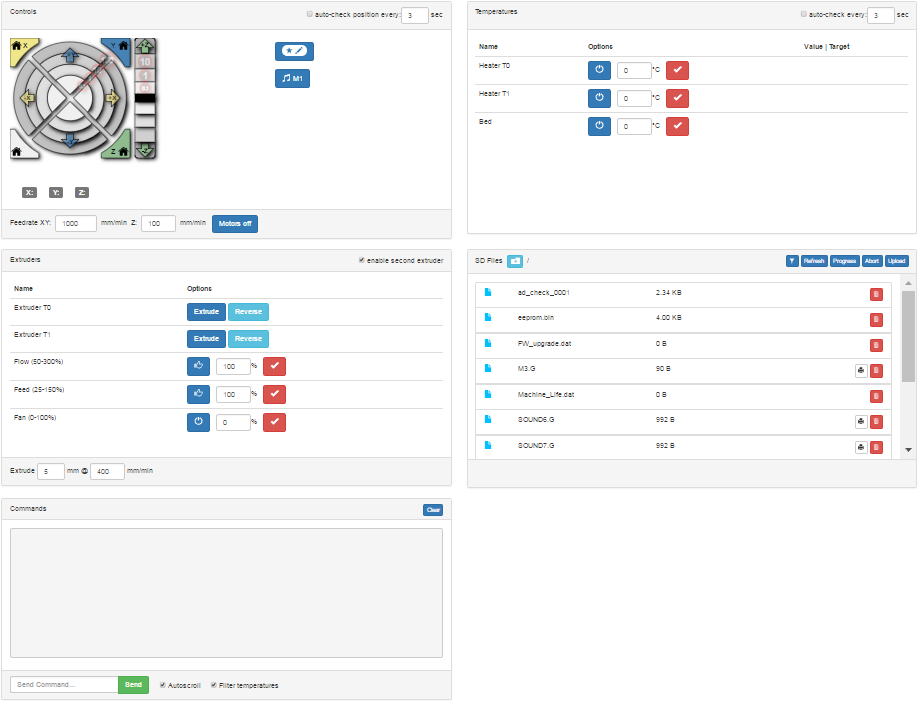
\includegraphics[scale=1.15,angle=0]{ESP3D_WebUI.png}
	\caption{Übersicht der Weboberfläche des ESP3D \cite{ESP3D_Web_UI}. Diese gilt nur als beispielhafte Ansicht, daher wird nicht detaillierter auf sie eingegangen.}
	\label{img:Weboberflaeche_ESP3D_Uebersicht}
\end{figure} 



\subsection{Human Machine System (HMS)}\label{subsec:HMS_SW}
Das \textit{Human Machine System} dient als Client des im Abschnitt \ref{subsec:WMU} beschriebenen Webservers. Es läuft auf allen Endgeräten welche sich im selben Netzwerk mit der \textit{Interface Controlling Unit} befinden und über eine Webbrowser Anwendung verfügen. 









\subsection{Printer Control Unit (PCU)}\label{subsec:PCU}
Die Software der \textit{Printer Control Unit} ist dafür zuständig den 3D-Druckprozess zu steuern. Die Druckinformationen werden dabei in Form von sogenanntem G-Code von einem CAD-Programm auf einem Computer geliefert. Dieser G-Code besteht aus verschiedensten Befehlen, welche in unterschiedlichen Produktionsmaschinen verwendet werden (z.B. CNC-Maschinen oder 3D-Drucker) \cite{G_Code_Tutorial}. Um G-Code in den eigentlichen 3D-Druckprozess umzusetzen, wird ein sogenannter G-Code Interpreter benötigt. Da es den Rahmen dieses Projekts sprengen würde einen eigenen Interpreter zu realisieren, wird eine bestehende Firmware (\textit{Marlin}) eingesetzt. 

Dieses kann über die beiden Files \textit{Configuration.h} und \textit{Configuration\_adv.h} auf die verwendete Hardware konfiguriert werden. Um die Einstellungen möglichst zu vereinfachen ist es von Vorteil die eigene Hardware mit der gleichen Pinbelegung zu realisieren wie ein bereits bestehendes und von \textit{Marlin} unterstütztes Board \cite{Marlin_Configuration}. 





